\documentclass{beamer}
\usepackage[utf8]{inputenc}
\usepackage{graphicx}
\usepackage{multicol}
\usepackage{booktabs}
\usepackage{tikz}
\usetikzlibrary{shapes.geometric, arrows}
\usepackage[x11names, rgb, dvipsnames]{xcolor}
\definecolor{SkyBlue}{HTML}{87CEEB}
\definecolor{LightOrange}{HTML}{FFA500} 
\definecolor{SteelBlue}{HTML}{4682B4}
\usetikzlibrary{shapes.geometric, arrows, trees}
\hyphenpenalty=10000
\exhyphenpenalty=10000

\begin{document}

% Prima diapositiva con solo sfondo
\begin{frame}
    \begin{tikzpicture}[remember picture, overlay]
        \node[opacity=0.85, at=(current page.center)] {
            
\includegraphics[width=\paperwidth,height=\paperheight]{sfondo.png}
        };
    \end{tikzpicture}

    \begin{center}
    \bigskip
        {\Huge \bfseries Synthetic Data Generation with Nonparametric Bayesian Methods}\\[0.5cm]
        {\Large \itshape Highlight privacy-preserving data analysis}\\[1cm]
    \end{center}

    % Autori
    \begin{flushleft}
        \textbf{Giovanni Mele, Chiara Noemi Nesti, Chiara Tomasini,\\Gianluca Villa, Andrea Violante, Stefano Zara}
    \end{flushleft}

    % Supervisore
    \begin{flushright}
        \textit{Supervised by:}\\
        Prof. Mario Beraha\\
        PhD researcher at Politecnico di Milano
    \end{flushright}
    
\end{frame}

############################################################

\section{Why Synthetic Data?}

\begin{frame}
\frametitle{The Role of Data in Society}
\begin{columns}[T] % [T] aligns columns at the top
    \begin{column}{0.6\textwidth}
        In today's data-driven world, sensitive information plays a crucial role in generating insights and making accurate predictions. However, its use also introduces significant privacy risks, including the potential for identity theft, highlighting the need for careful handling and protection.
        
        \begin{center}
            \textbf{\textit{\\How can we harness the power of sensitive data to drive innovation and inform decisions, while ensuring privacy and ethical use?}}
        \end{center}
        
    \end{column}
    \begin{column}{0.4\textwidth}
        \begin{figure}
            \centering
            \bigskip
            \medskip
            
\includegraphics[width=\linewidth]{slide2.png}
        \end{figure}
    \end{column}
\end{columns}
\end{frame}

#####

\begin{frame}{Differential privacy}
\begin{figure}
        \centering
        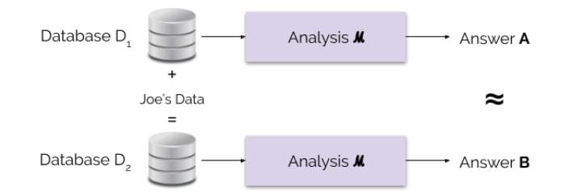
\includegraphics[width=0.8\linewidth]{DP1.png}
    \end{figure}
    \vspace{0.5cm} % Aggiunge spazio tra le immagini
    
    Differential privacy consists in releasing statistical information about datasets while protecting the privacy. This is done by adding some noise.

\end{frame}
####

\begin{frame}
\frametitle{Goals:}
\centering
\begin{tikzpicture}

\node[draw, fill=SkyBlue, text width=5cm, align=center, rounded corners, minimum height=2cm, drop shadow={shadow xshift=0.5ex,shadow yshift=-0.5ex}] (A) at (0,0) {\textbf{ORIGINAL DATASET} \\ \small It contains valuable information};

% Secondo box (SYNTHETIC DATA)
\node[draw, fill=LightOrange, text width=9cm, align=center, rounded corners, minimum height=2cm, drop shadow={shadow xshift=0.5ex,shadow yshift=-0.5ex}] (B) at (0,-3) {\textbf{SYNTHETIC DATASET} \\ \small It preserves the essential characteristics and patterns of the original data but modifies the sensitive elements, providing a safer alternative};

\draw[->, thick=4.5, color=black] (A) -- (B);
\end{tikzpicture}

\vspace{0.3cm}

\begin{center}
\textit{The fundamental goal is to simulate synthetic data while preserving real patterns while minimizing privacy risks.}
\end{center}
\end{frame}

############################################################

\section{Pólya Tree Processes}
\begin{frame}{Pólya Tree}


A Pólya tree defines a prior distribution on function spaces by recursively partitioning the interval $[0, 1]$ into subintervals. Probabilities are assigned to these subintervals using Beta-distributed random variables. This recursive partitioning process helps define a flexible and rich class of distributions, allowing for complex modeling of uncertainty in function spaces.
\bigskip % Spazio verticale tra il grafico e il testo

\begin{center}
    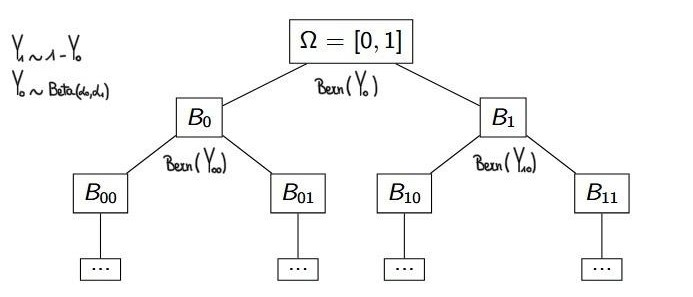
\includegraphics[width=\textwidth]{albero.jpg}
    
\end{center}

\end{frame}

######
\begin{frame}{Pólya Tree Framework: Definitions and Parameterization}

    A Pólya tree is denoted by \textbf{\(G \sim \mathcal{PT}(\Pi, \mathcal{A})\)}\\
    \bigskip
    Lavine (1992) proposed the following choice
    to center the \(\mathcal{PT}\) around a given centering probability measure \(G_0\). \\ 
    In short, fix \(\Pi\) as
     the dyadic quantiles of \(G_0\) and use \(\alpha_{\epsilon_0}=\alpha_{\epsilon_1}\) for every level.\\
     \bigskip
     Lavine (1992) proposes \(\alpha_{\epsilon_0 ... \epsilon_m} = m^2\) as a canonical choice. Walker and Mallick (1997) and Paddock (1999) updated the model by defining  \(\alpha_{\epsilon_0 ... \epsilon_m} = c \cdot m^2\), with \(c > 0\). \\
     \bigskip
     The posterior distribution of a Pólya Tree remains a Pólya Tree. \\
    This is due to the conjugacy property of the model in fact the structure is preserved after updating with observed data.

     
\end{frame}

######

\begin{frame}{Data Generation and Pólya Tree Modeling}
\begin{minipage}{0.5\textwidth}
    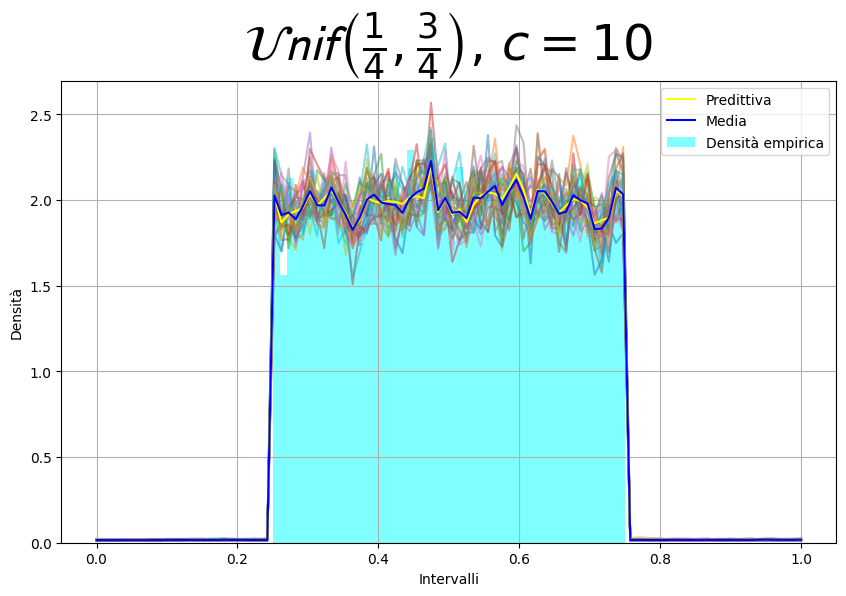
\includegraphics[width=\textwidth]{Unif1.png}

    \bigskip
    
    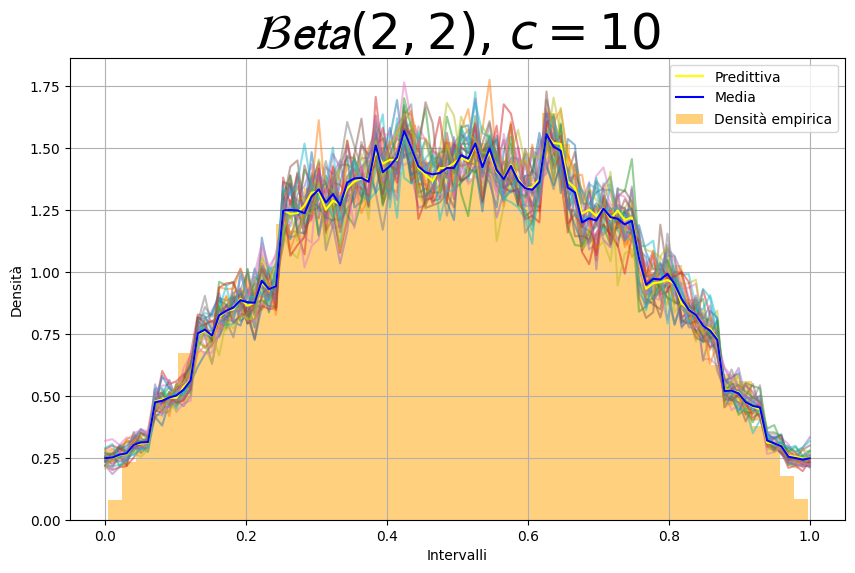
\includegraphics[width=\textwidth]{Gaus1.png}

  \end{minipage}
  \hfill
  \begin{minipage}{0.45\textwidth}
    We defined the prior as a Pólya tree with depth \( M = 10 \) and parameters \( \alpha = c \cdot m^2 \), with \( c \) being a fixed constant. \\
    
    After calculating the posterior distribution, we sampled 30 distributions from it.
  \end{minipage}
\end{frame}
#####

\begin{frame}{Initial Predictive Analysis}
\centering
    \begin{minipage}{0.7\textwidth}
        \centering
        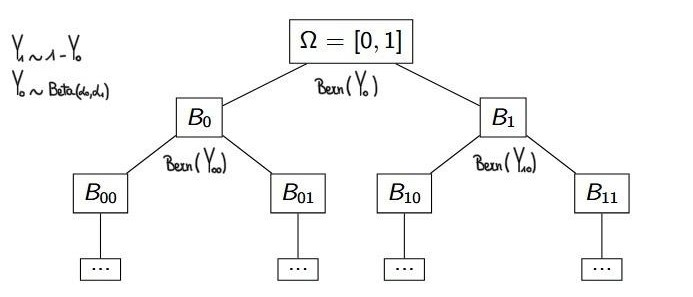
\includegraphics[width=\textwidth]{albero.jpg}
        \smallskip % Spazio tra le due immagini
    \end{minipage}

    \begin{minipage}{0.65\textwidth}
        \centering
        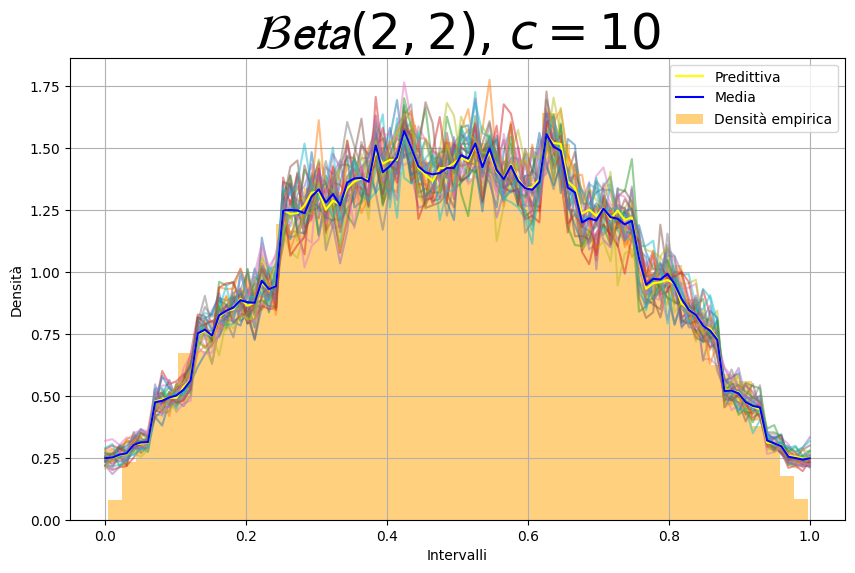
\includegraphics[width=\textwidth]{Gaus1.png}
    \end{minipage}
\end{frame}#####

###########################################################
\section{Cosa succede al variare di c}
\begin{frame}{Exploring the Sensitivity to Parameter \(c\)}
    \centering
    % Prima riga di immagini
    \begin{figure}
        \begin{minipage}{0.32\textwidth}
            \centering
            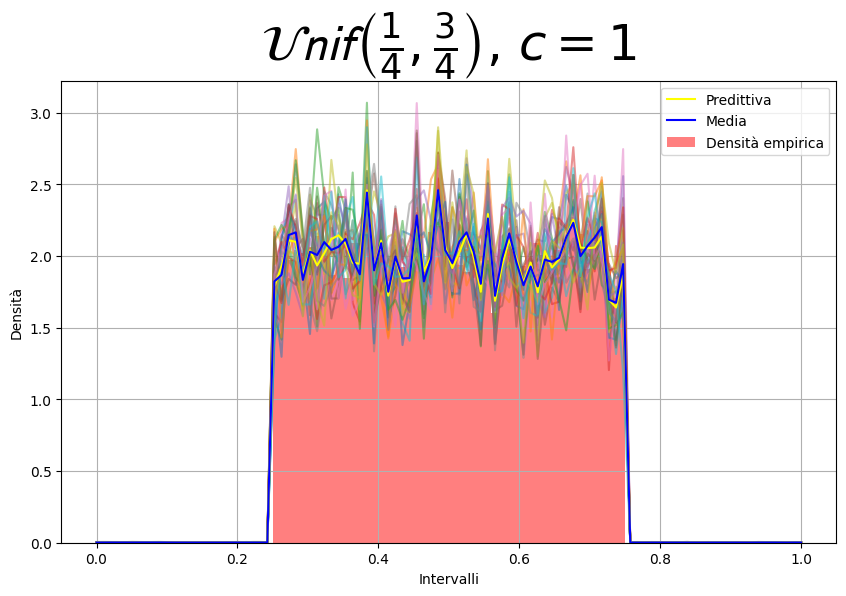
\includegraphics[width=\textwidth]{Unifc1.png}
        \end{minipage}
        \hfill
        \begin{minipage}{0.32\textwidth}
            \centering
            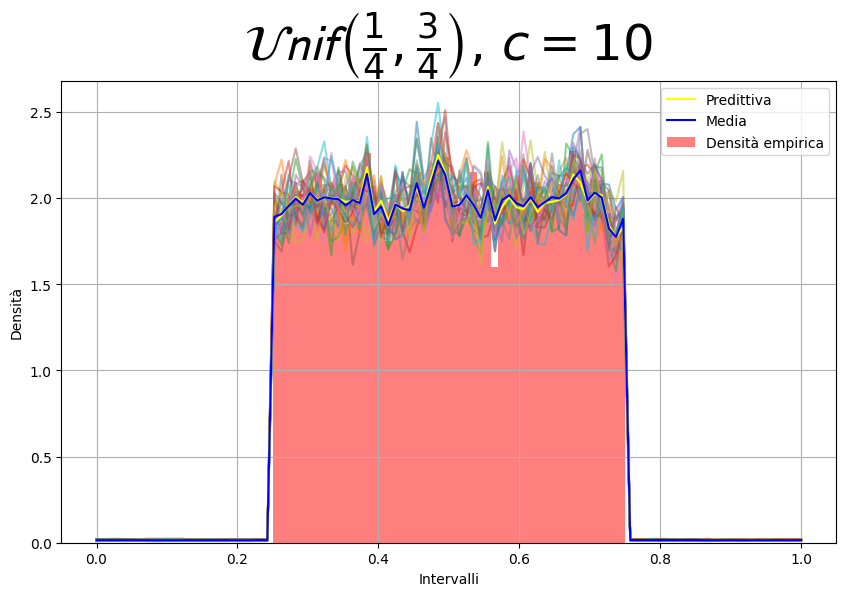
\includegraphics[width=\textwidth]{Unifc10.png}
        \end{minipage}
        \hfill
        \begin{minipage}{0.32\textwidth}
            \centering
            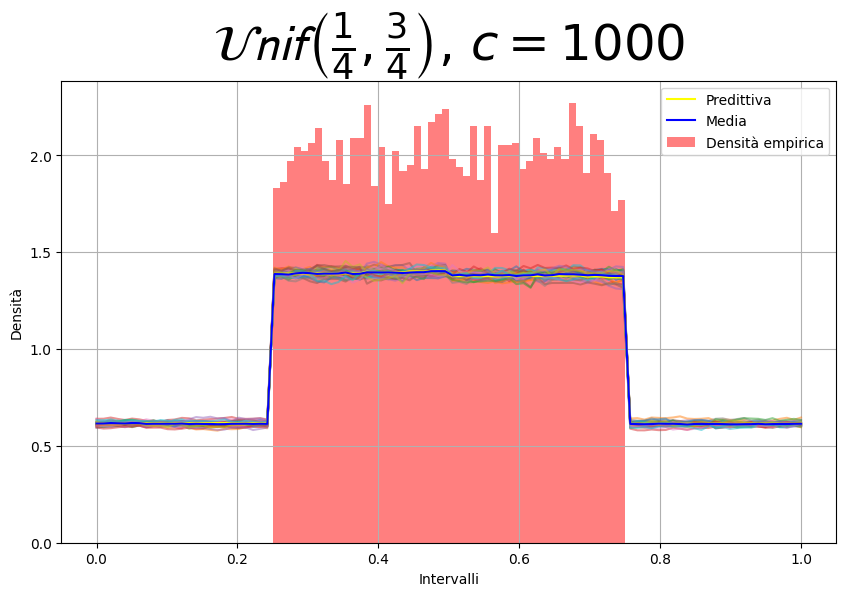
\includegraphics[width=\textwidth]{Unifc1000.png}
        \end{minipage}
    \end{figure}
    \caption{\(Unif(1/4,3/4)\)}

\bigskip
    % Seconda riga di immagini
    \begin{figure}
        \begin{minipage}{0.32\textwidth}
            \centering
            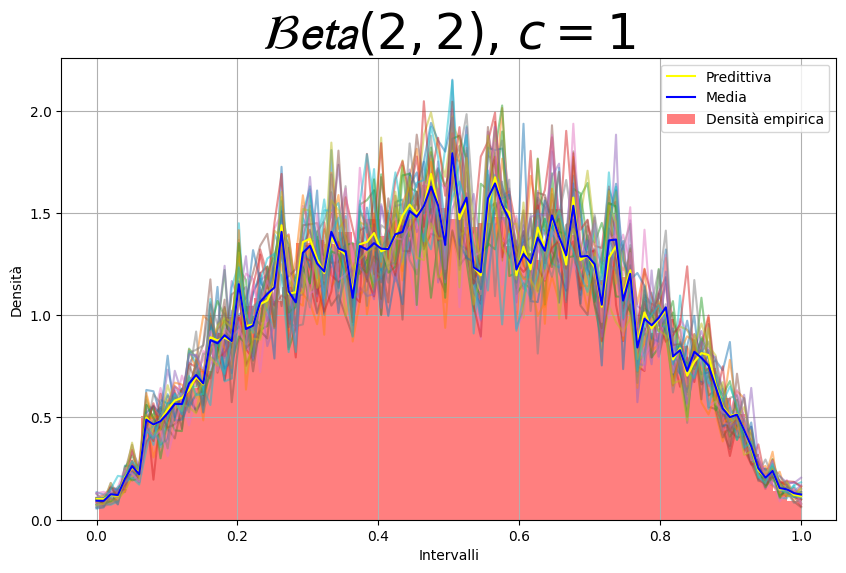
\includegraphics[width=\textwidth]{Betac1.png}
        \end{minipage}
        \hfill
        \begin{minipage}{0.32\textwidth}
            \centering
            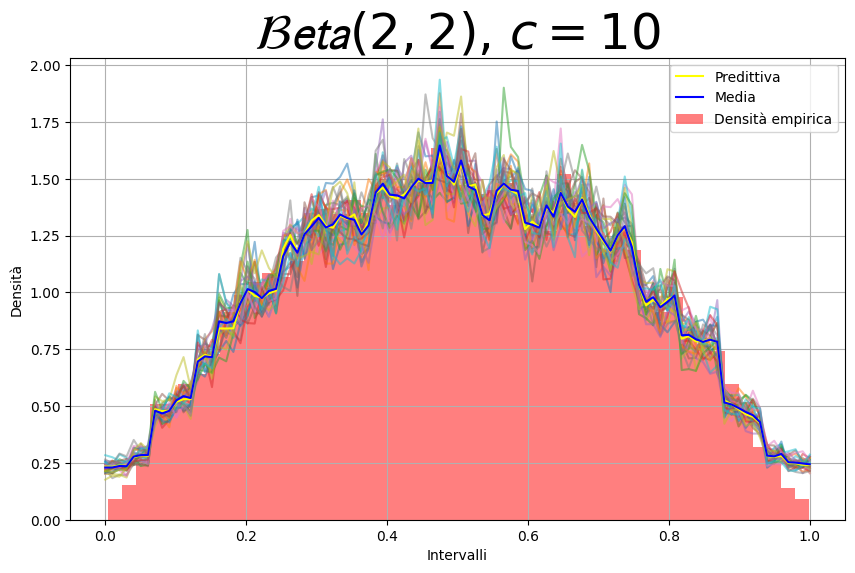
\includegraphics[width=\textwidth]{Betac10.png}
        \end{minipage}
        \hfill
        \begin{minipage}{0.32\textwidth}
            \centering
            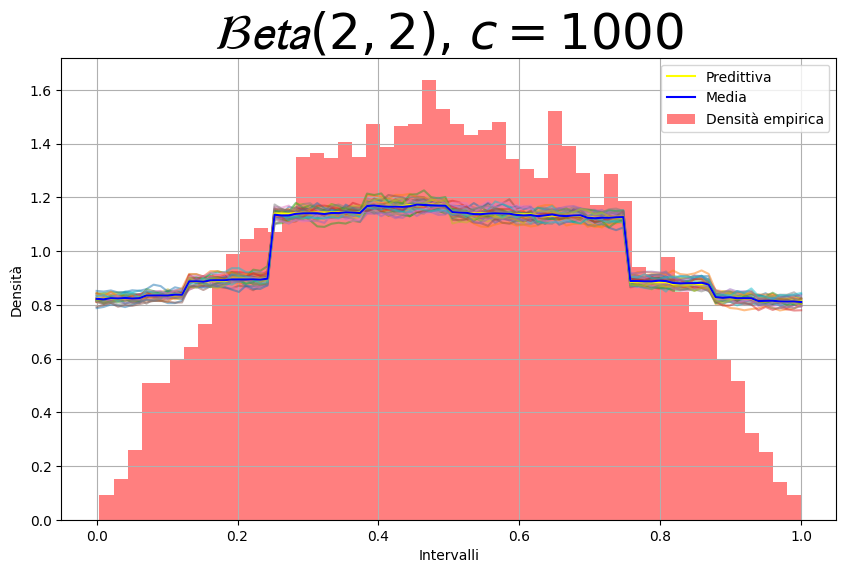
\includegraphics[width=\textwidth]{Betac1000.png}
        \end{minipage}
    \end{figure}
    \caption{\(Beta(2,2)\)}
\end{frame}


\begin{frame}{Analyzing the Optimal Choice for Parameter \(c\)}
    \centering
    \begin{minipage}{0.45\textwidth}
        \centering
        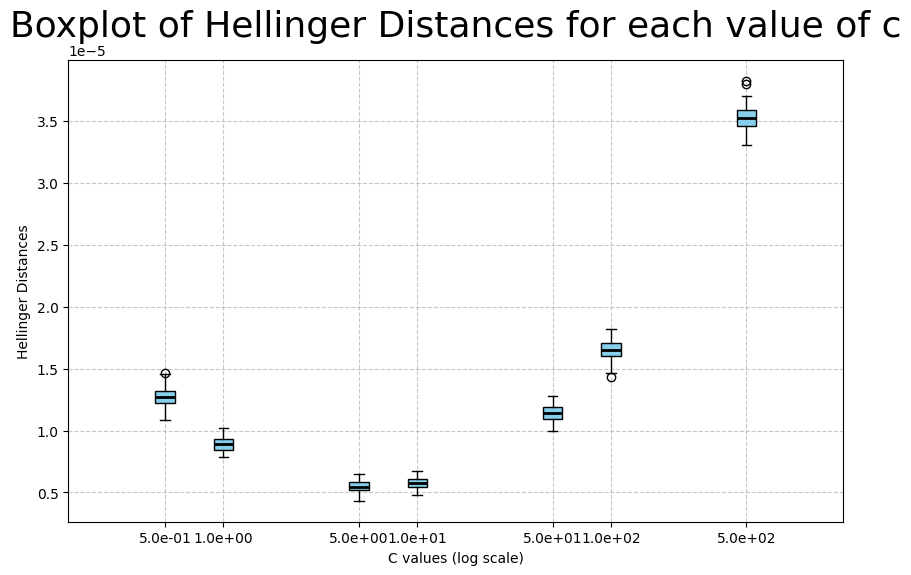
\includegraphics[width=\textwidth]{sorriso.jpeg}
    \end{minipage}
    \hfill
    \begin{minipage}{0.45\textwidth}
        \centering
        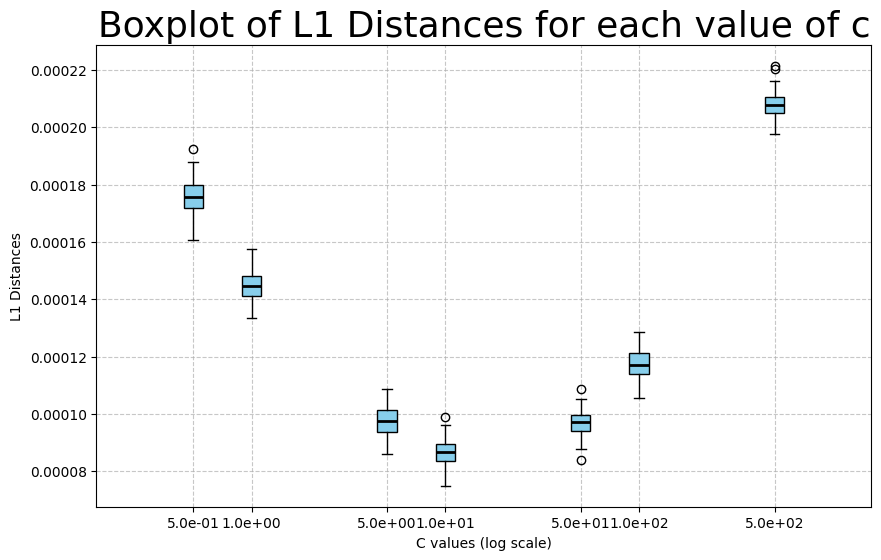
\includegraphics[width=\textwidth]{sorriso2.jpg}
    \end{minipage}
    
    \bigskip
    \bigskip
    A higher \(c\) leads to greater adherence to the prior, reducing variability, while a lower \(c\) allows for more flexibility, enabling exploration of diverse distributions. Its choice affects the trade-off between prior belief and adaptability to observed data, particularly as the tree depth increases.
    
\end{frame}

##########################################################

\section{Controllo correttezza}
\begin{frame}{Accuracy of Our Prediction}
        \centering
    % Prima riga di immagini
    \begin{figure}
        \begin{minipage}{0.32\textwidth}
            \centering
            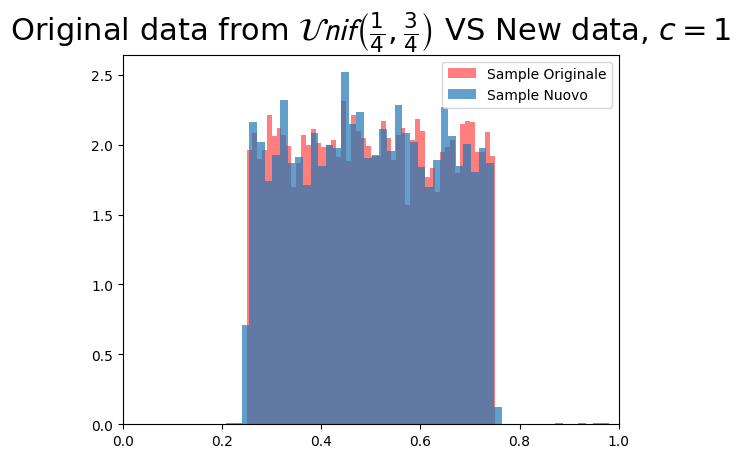
\includegraphics[width=\textwidth]{Predc1.png}
        \end{minipage}
        \hfill
        \begin{minipage}{0.32\textwidth}
            \centering
            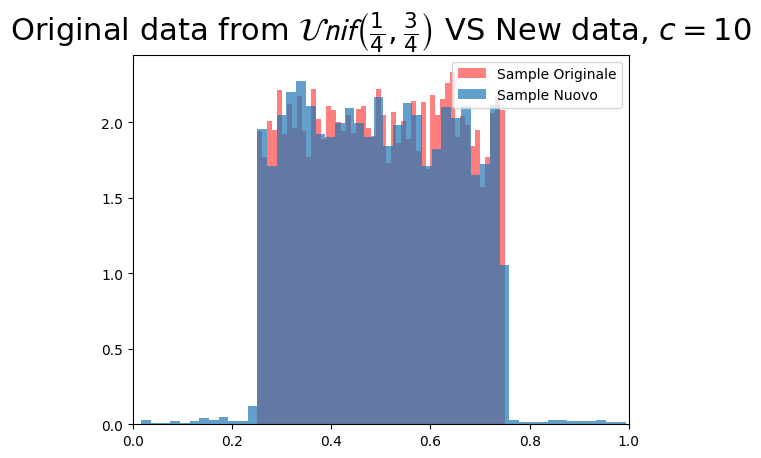
\includegraphics[width=\textwidth]{Predc10.png}
        \end{minipage}
        \hfill
        \begin{minipage}{0.32\textwidth}
            \centering
            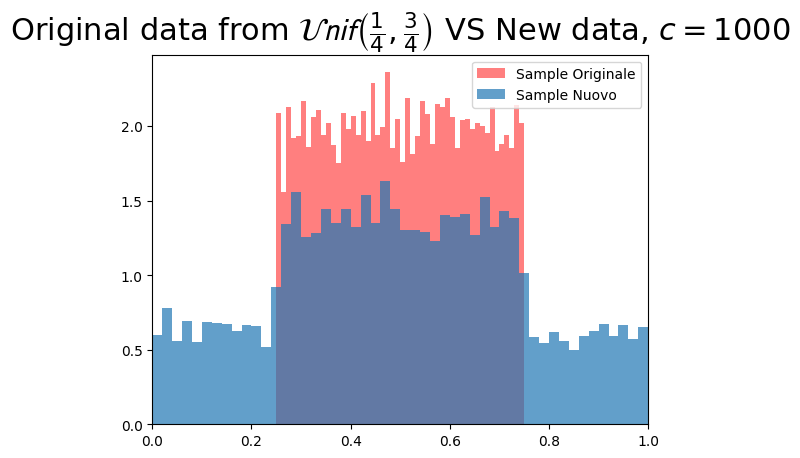
\includegraphics[width=\textwidth]{Predc1000.png}
        \end{minipage}
    \end{figure}
    \caption{Predictive density estimated for an \(Unif(1/4,3/4)\)}

\bigskip
    % Seconda riga di immagini
    \begin{figure}
        \begin{minipage}{0.32\textwidth}
            \centering
            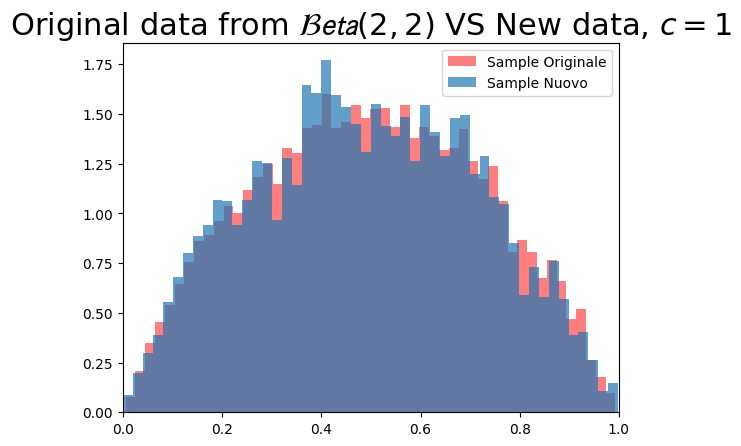
\includegraphics[width=\textwidth]{PredBetac1.png}
        \end{minipage}
        \hfill
        \begin{minipage}{0.32\textwidth}
            \centering
            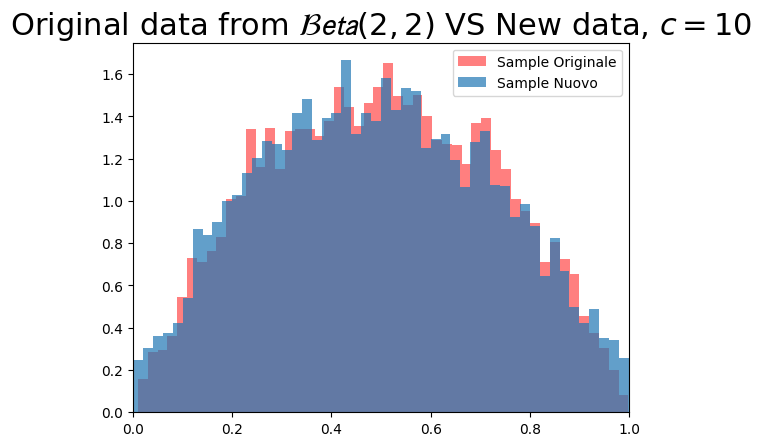
\includegraphics[width=\textwidth]{PredBetac10.png}
        \end{minipage}
        \hfill
        \begin{minipage}{0.32\textwidth}
            \centering
            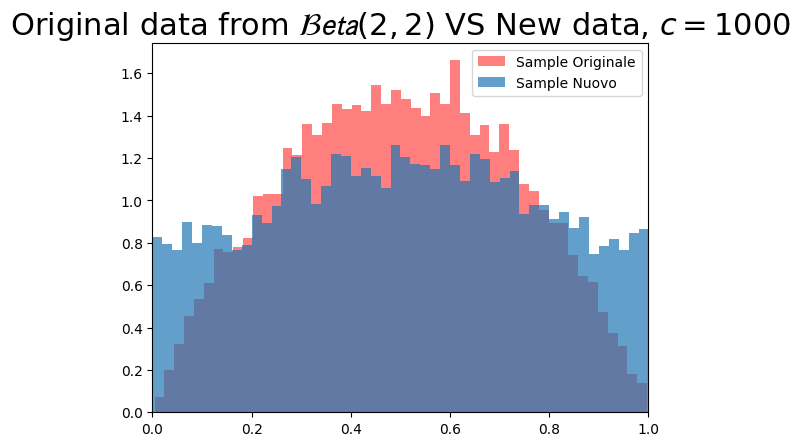
\includegraphics[width=\textwidth]{PredBetac1000.png}
        \end{minipage}
    \end{figure}
    \caption{Predictive density estimated for a \(Beta(2,2)\)}

\end{frame}

\end{document}